\documentclass[14pt,aspectratio=169,hyperref={pdftex,unicode},xcolor=dvipsnames]{beamer}
\usepackage[english,russian]{babel}
\usepackage[utf8x]{inputenc}
\usepackage[T2A]{fontenc}
\usepackage{cmap}
\usepackage{paratype}
\usepackage{minted} % для примеров кода (требует параметра -shell-escape)

\usetheme{metropolis}
\usefonttheme[]{professionalfonts}  % запрещаем beamer'у перезаписывать мат. шрифты
\metroset{numbering=fraction}
\metroset{subsectionpage=progressbar}

\setbeamercolor{frametitle}{fg=black}
\setbeamertemplate{frametitle}
{
 \vspace{3mm}\insertframetitle\par
}
\setbeamertemplate{title separator}{}
\setbeamertemplate{footnote separator}{}


\usebackgroundtemplate{
\includegraphics[width=\paperwidth,height=\paperheight]{./common/background_white.jpg}}

\logo{\vspace{-1.2cm}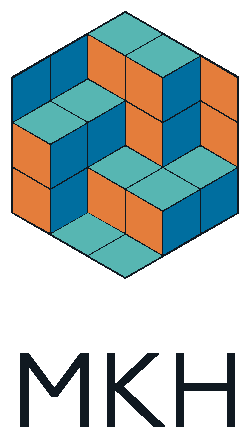
\includegraphics[width=6mm]{./common/short-v.pdf}\hspace*{1.08\textwidth}}

\institute
{
  \begin{columns}
    \begin{column}{1.5cm}
    
\includegraphics[height=15mm,keepaspectratio]{./common/math-cs.pdf}
    \end{column}
    \begin{column}{4cm}
          Faculty of mathematics and computer science SPBU
    \end{column}
  \end{columns}
}


\begin{document}

\begin{frame}[plain]
  \begin{center}
    \textbf{Ogloblin Ivan Semenovich}

    {\Large\textbf{ Study of the effect of noise on efficient quantum search algorithms}}

     {\small June 2022 course work}

    {\small Scientific adviser: Tikhomirov Sergei Borisovich}

  \end{center}


  \begin{columns}
    \begin{column}{1cm}
    
\includegraphics[height=15mm,keepaspectratio]{./common/math-cs.pdf}
    \end{column}
    \begin{column}{10cm}
      \small
          Faculty of mathematics and computer science SPBU\\
          Specialty <<modern programming>>
    \end{column}
  \end{columns}
\end{frame}



\begin{frame}
\frametitle{Introduction}

\begin{itemize}
\item The errors resulting from noisy quantum gates and decoherence make quantum devices far from perfect
\item NISQ era algorithms strive for shallow depth to reduce the impact of noise from environment\footnote{\href{https://arxiv.org/abs/2101.08448}{Noisy intermediate-scale quantum (NISQ) algorithms}}
\item There are three different strategies to improve accuracy and efficiency
of the Grover’s search algorithm on the NISQ processors\footnote{\href{https://doi.org/10.1007/s11128-021-03165-2}{Zhang, K., Rao, P., Yu, K., Lim, H., \& Korepin, V. (2021)}}\\
\end{itemize}


\end{frame}

\begin{frame}
\frametitle{The problem}
\begin{enumerate}
\item Implement the algorithm improvements described in the article
\item Create an environment for testing different variations of the algorithm with different noise models and different number of qubits
\item Conduct a series of experiments and explore noise impact on variations of the algorithm
\end{enumerate}
\end{frame}

\begin{frame}{Implementation}
	\begin{itemize}
		\item Using Qiskit and IBMQ\footnote{\href{https://github.com/StudioShader/QPSA}{public repository}}
		\item Using thermal relaxation  model\footnote{\href{https://github.com/Qiskit/qiskit-tutorials/blob/master/tutorials/simulators/3_building_noise_models.ipynb}{qiskit thermal relaxation noise model}}
		\item Error coupling map on qubits as on the real device "Melbourne"
		\item Toffoli gate implementation through Qiskit function .mct()\footnote{\href{https://qiskit.org/documentation/stubs/qiskit.circuit.QuantumCircuit.mct.html}{.mct() function}}
	\end{itemize}
\end{frame}

\begin{frame}{Tests on 6 qubits\footnote{as the noise parameter increases, the amount of noise decreases. At 1 it simulates noise as on the real device}}
	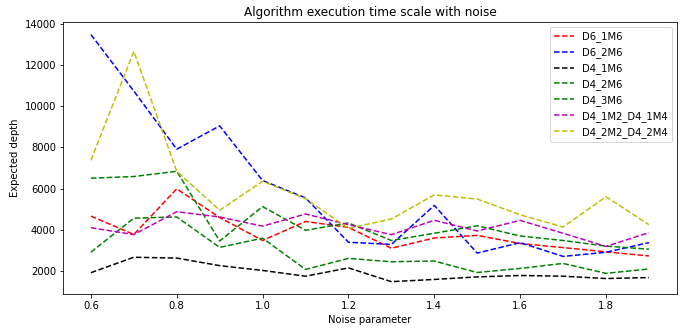
\includegraphics[width=13cm]{images/6_qubit_tests_.png}
\end{frame}

\begin{frame}{Tests on 6 qubits: results}
	\begin{itemize}
		\item Dm\_iM6 stands for algoritm with local Grover operator applied $i$ times
		\item We can see that some algorithms perform better than the others
		\item Some algorithms scale better with noise parameter. D6\_2M6 has lower expected depth than D4\_1M2\_D4\_1M4 at low noise parameter values, but greater at large noise parameter values
	\end{itemize}
\end{frame}

\begin{frame}{Tests on 8 qubits}
		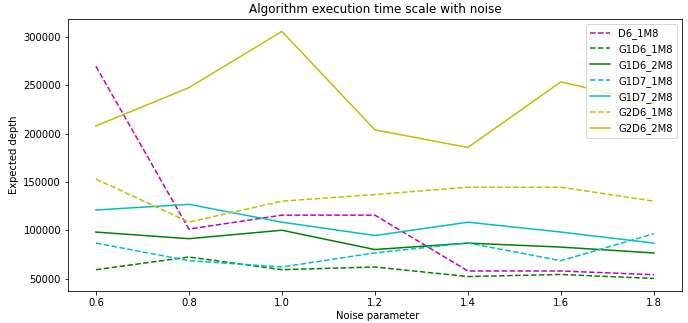
\includegraphics[width=14cm]{images/8_qubit_tests1.png}
\end{frame}

\begin{frame}{Tests on 8 qubits}
	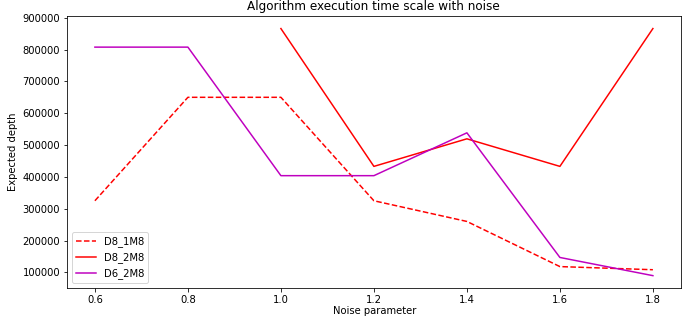
\includegraphics[width=14cm]{images/8_qubit_tests2.png}
\end{frame}

\begin{frame}{Tests on 8 qubits: results}
	\begin{itemize}	
		\item the number of Grover operator calls for 8 qubits should be ${\frac{\Pi\sqrt{2^8}}{4}} \approx 12$
		\item with such number of Grover operators it already takes much time to test an algorithm. Not only because of it's depth, but also because of the large minimum sufficient number of shots. And it is basically useless to test an algorithm with more than four Grover operators, because the result won't be much different from pure noise
		\item All tests were done on intel i5 8th gen processor 
	\end{itemize}	
\end{frame}

\begin{frame}{Noise parameter}
	Noise parameter scales the constants T1 and T2 in thermal relaxation noise model\footnote{\href{https://arxiv.org/pdf/2101.02109.pdf}{T1/T2 thermal relaxation noise model}}. This parameter describes the physical ability to store and apply operations on qubits without unnecessary noise. In order to find minimum sufficient value for the noise parameter, we want to test algorithms on different number of qubits and much more different values of noise parameter. 
\end{frame}

\begin{frame}{10 qubit tests}
	 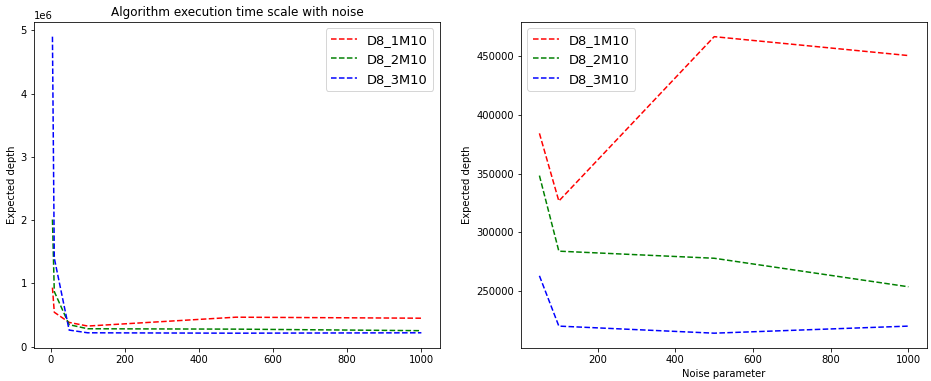
\includegraphics[width=14cm]{images/10_qubit_tests.png}
\end{frame}

\begin{frame}{10 qubit tests: results}
	\begin{itemize}
		\item There is a definite value of noise parameter, after which there is no visible decrease of expected depth. We want to know how this value scales with the number of qubits
		\item Unfortunately we only have so much processing power, it barely reaches the 10th qubit front. Further experiments should be carried out on processors more adapted for such quantum simulations
	\end{itemize}
\end{frame}

\begin{frame}[noframenumbering, plain]
\frametitle{Summary}

\begin{itemize}
\item We implemented a useful playground for tests with different noise models
\item Conducted a set of experiments to show limitations of efficient quantum search algorithm
\end{itemize}

\vspace{5mm}\hrule\vspace{5mm}

\begin{center}
Ivan Ogloblin\\
studioshader2018@gmail.com \\
\href{https://github.com/StudioShader/QPSA}{\textcolor{blue}{github repository}}
\end{center}

\end{frame}

\end{document}
